\chapter{Methods}

\begin{comment}
\section{{Protocol:First Part}
\begin{itemize}
\item 5 jumps
\item lie down on \textbf{prone} position
\item 5 jumps
\item lie down on \textbf{left side} position
\item 5 jumps
\item lie down on \textbf{supine} position
\item 5 jumps
\item lie down on \textbf{right side} position
\end{itemize}


\section{Data Collection Protocol}





The aim of this protocol is to collect data with the two mattresses (SensigTex under the Sensomative) of different heart rates and breath rates.
During this protocol will be asked to change positions to collect the data in all four positions: supine position, lateral right position, prone position, and lateral left position.
Before data collection will also record what the sensors measure in case a participant is not on the mattress whether it is stationary or moving.




\section{Experimental Setting}
The experimental setting includes a bed above which two sensors will be positioned: SensingTex and Sensomative. The Sensomative has to be placed under the  SensingTex Sensor and the sensor will be used simultaneously. 
\subsection{Mattress }
The Sensomative Sensor gives the best result for detecting breath rate and heart rate when placed under the chest.[\textbf{investigate possible distance from the start of the mattress}] For this reason, should be placed exactly []cm from the top part of the mattress.
Above this sensor, the SensingTex Sensor should be placed above this sensor because applying even pressure will not affect the measurements.
\subsection{Pillow and bed sheets}

\subsection{Ground truth }
The ground truth value for this data collection will be collected via polysomnography and video cameras. Polysomnography allows to recording this following parameters:

\begin{itemize}
    \item Nasal flow and nasal pressure: that will be used as the ground truth for the breath rate.
    \item Chest and abdomen movement: that can be also used as ground truth for the breath rate, with different types of approaches. [\textbf{can also detect the heart rate o heart movement?}]
    \item SPO2 and Pulse with a fingertip: that will be the ground truth data for the heart rate
    \item \{ Raimon \} 
\end{itemize}

Along with Polysomnography will also be involved cameras to record the position of the participant for further analysis.

\section{Patient setting}
\subsection{what to wear}
The participant should wear comfortable clothes. T-shirts are recommended in order not to have a too high layer of fabric that could interfere with the detection of data, in particular with the heart bit detection.
\subsection{Lay down position}
There are four different positions that will be asked to\begin{itemize}
    \item Lateral left position
    \item Lateral right position
    \item Prone
    \item Supine
\end{itemize}
\subsection{Pattern Position}
One of this data collection's main points is finding peaks in different positions, so each patient will be asked to lay down in a different position pattern.
\begin{itemize}
    \item supine position, lateral right position, prone position, and lateral left position
    \item lateral right position, prone position, lateral left position and supine position
    \item prone position, lateral left position, supine position and lateral right position
    \item lateral left position, supine position, lateral right position and prone position
\end{itemize}
Once a position pattern is given to a specific participant, it must be repeated for each step of the protocol.
\subsection{how long they have to lay down}





\section{Data Collection}
\subsection{Joint Data Collection}
\subsubsection{Breathing rate and Heart rate at rest in normal condition}
In this part of the protocol, the aim is to collect data on the breathing rate and heart rate of the participants at rest.
\subsubsection{Breathing rate and Heart rate at rest during mattress movement}
This part of the protocol aims to collect data on the participant's breathing rate and heart rate at rest while the mattress is moving.
\subsubsection{Breathing rate and Heart rate after an effort}
In this part of the protocol, the aim is to collect data on the participant's breathing rate and heart rate after an effort, to analyze data of an accelerated breath and heart bit and gradually decelerated.
The effort consisted of ten jumping jacks repeated before each position change.

%\section*{Breath Rate}



\subsection{Heart Rate Data Collection}
\subsubsection{Heart rate at rest with constrained breath rate}
This part of the protocol aims to provide a known rhythm to the breath rate according to an acoustic time. The sound will indicate when they start to inhale and exhale to the participants.

\subsubsection{Heart rate at rest with constrained breath rate during mattress movement}
This part of the protocol aims to provide a known rhythm to the breath rate according to an acoustic time while the mattress is moving. The sound will indicate when they start to inhale and exhale to the participants.

\end{comment}

\section{Instruments}
\subsection{Sensomative}

\begin{figure}[h]
    \centering
    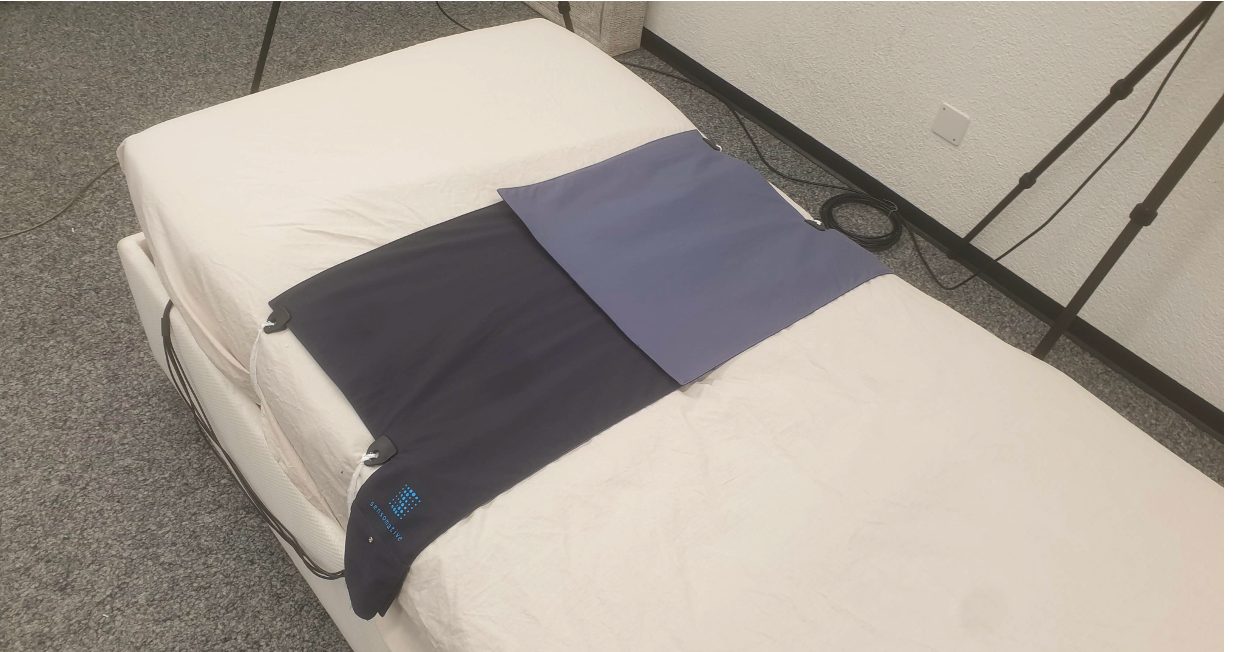
\includegraphics[width=0.5\textwidth]{img/sensomative.png}
    \caption{Sensomative over a bed}
    \label{fig:sensomativeBed}
\end{figure}

\subsection{SensingTex}
\begin{figure}[h]
    \centering
    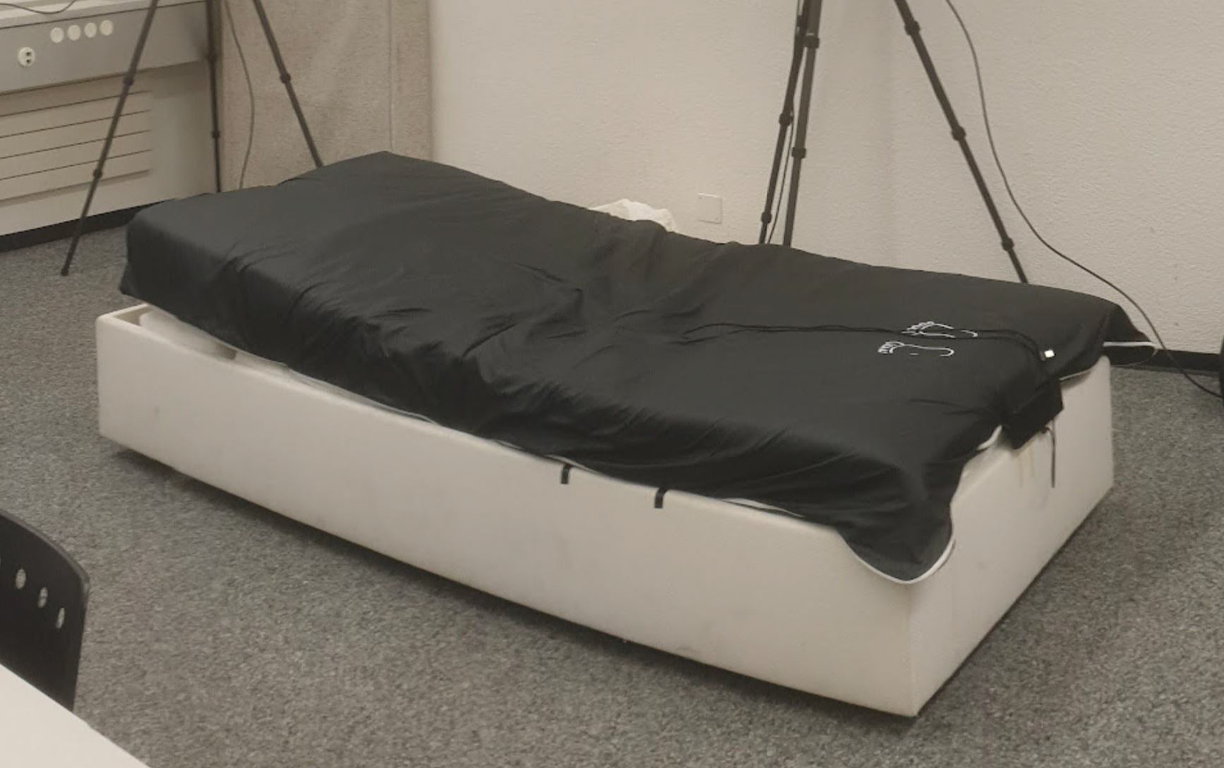
\includegraphics[width=0.5\textwidth]{img/sensingtex.png}
    \caption{Sensomative over a bed}
    \label{fig:sensingtex}
\end{figure}

\begin{figure}[h]
    \centering
    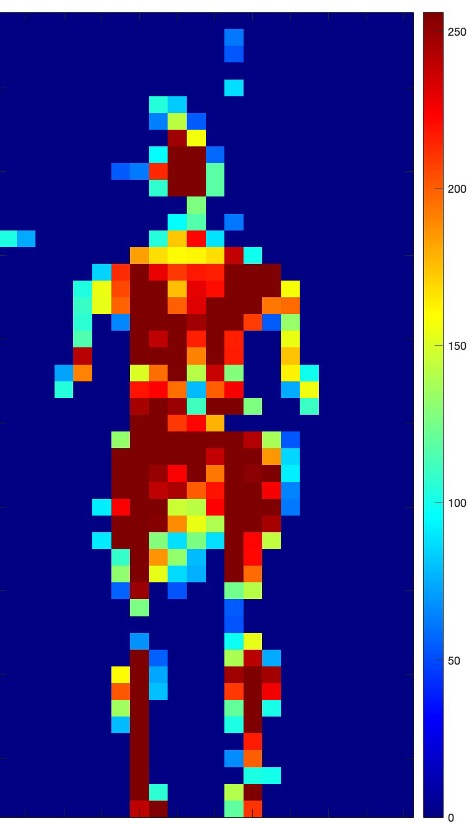
\includegraphics[width=0.5\textwidth]{img/sensingtex_2.jpg}
    \caption{Sensomative over a bed}
    \label{fig:sensingtexData}
\end{figure}


\section{Nox A1, polysomnography}
For this reason, this thesis aims to study the possibility to use an unobtrusive sensor placed over the usual mattress to retrieve 
respiratory rate without discomfort for the person lying down on it. 


The sensors in this project appear like a thin mattress similar in size to a common one that can be easily installed with adjustable straps.
In particular, the sensors are pressure-sensor textiles from \textit{SensingTex®}; in our case, was used the Pressure Mat Dev Kit,
 that has a sensor area of 192 x 94 cm filled with 1056 sensors (hereafter also referred to as "Channels") sampled at 250hz
 with a total sensor area density of 4 sensors for 10cm$^2$.
 The raw data extracted from the mattress can be viewed together to visually see the position of the person since the sensors are pressure sensors
the different pressures exerted by the presence/absence of a body on it or by its parts are given as a number inside an interval. 
So it is possible to create a heat map (or heatmap) to show the variation in colour of the intensity of the pressure, which can create the shape of
a person on the mattress.

Looking closer into signals of singles channels is possible to see a pattern that resembles a breathing rhythm,  similar to the data that can
 be retrieved from the nasal pressure exerted on the cannula of cardiorespiratory polysomnography.
This pattern was the key factor in deciding to use this sensor mattress (hereafter also referred to as "Sensor Mat" or "Mat"). 
In the laboratory where this project was carried on, was available a rocking bed (Somnomat) involved in a study of an intervention for 
sleep apnea, it was decided to address another question or if it is possible to retrieve the respiratory rate while the rocking bed is moving.
The possibility of integrating SensingTex® with Somnomat could be significant to have a closer and faster intervention on sleep apnea.
\subsection{Somnomat}
\section{Preliminary Study of different approaches} 
\section{Data Collection}
\subsection{Normal Bed}
\subsection{Rocking Bed}

The primary objective of this study is to collect data to understand the feasibility of extracting breath rate from the mat; the second goal is to understand if the movement of the rocking bed could influence the signal.
The participant involved was 6, half male and half female, between 20-30 years old, who were asked to lie on a standard mattress covered with the sensor mattresses in a specific position. 
After the 4 minutes, they were asked to turn around in another position following a specific pattern: supine, left side, prone, right side.
Each participant wore a cardiorespiratory wireless and portable polysomnography device (Nox A1 PSG of Nox Medical) that was
monitoring respiratory inductance plethysmography (RIP) which is a method of evaluating pulmonary ventilation by measuring the movement of the chest and abdominal wall, nasal pressure, pulse and heart rate with ECG. 
The study was divided into two phases:

The setting for the first phase involves the pressure mat over a standard bed. During the night and through the different sleep stages, the breath rate increase or decreases, so we decide to insert a similar variability in our data. We asked the participant to perform a set of five jumps before lying down, so they performed a total of 20 jumps.
The setting for the second phase, since in this part we want to collect the data while the Somnomat is moving, we fixed the period for the movement of the bed at 4 seconds (15 periods in a minute) with an acceleration of 0.25 $m/s^2$. Also, for this phase, they have been asked to turn around following the specific pattern: supine, left side, prone, right side.
This results in a recording of 32 minutes long for each participant divided into 4 minutes in each of the 4 positions with normal bed and with Somnomat.

